%!TEX root = ../luanvan.tex
\chapter{Xây dựng hệ thống}

\section{Mô tả bài toán}

Hiện nay, việc quản lý VBCC được quy định cụ thể riêng theo từng Trường, nhằm hướng dẫn việc thực hiện, báo cáo, lưu trữ hồ sơ và phân cấp chịu trách nhiệm của cá nhân và đơn vị liên quan trong khi thực hiện công việc.
Tuy nhiên, công việc quản lý VBCC có nhiều hồ sơ, quy trình như bàn giao, in phôi VBCC, trình ký và đóng dấu, rà soát thông tin in lên phôi VBCC, lập sổ gốc, quản lý phát VBCC, xác minh VBCC, \ldots. còn thủ công nên ảnh hưởng chất lượng hiệu quả công việc.
Chẳng hạn như VBCC phát cho sinh viên dễ sai sót, do VBCC phải được in thông tin, ký tên, đóng dấu. Thông tin VBCC gồm có: số hiệu phôi, số vào sổ gốc, họ tên, ngày sinh, giới tính, nơi sinh, kết quả, ngày cấp, người cấp. 

Do đó, bài toán đặt ra nhu cầu cải tiến trong quản lý thông tin của người cấp, người được cấp và VBCC; số hóa các quy trình cấp VBCC, sở hữu VBCC, chia sẻ thông tin xác thực VBCC có liên quan đến thông tin cá nhân của người được cấp VBCC theo các quy định hiện hành về bảo vệ bí mật thông tin trong môi trường trực tuyến.

Quy trình quản lý VBCC ứng dụng blockchain được mô tả ở hình \ref{fig:vbcc}

\begin{figure}[htbp]
\centering
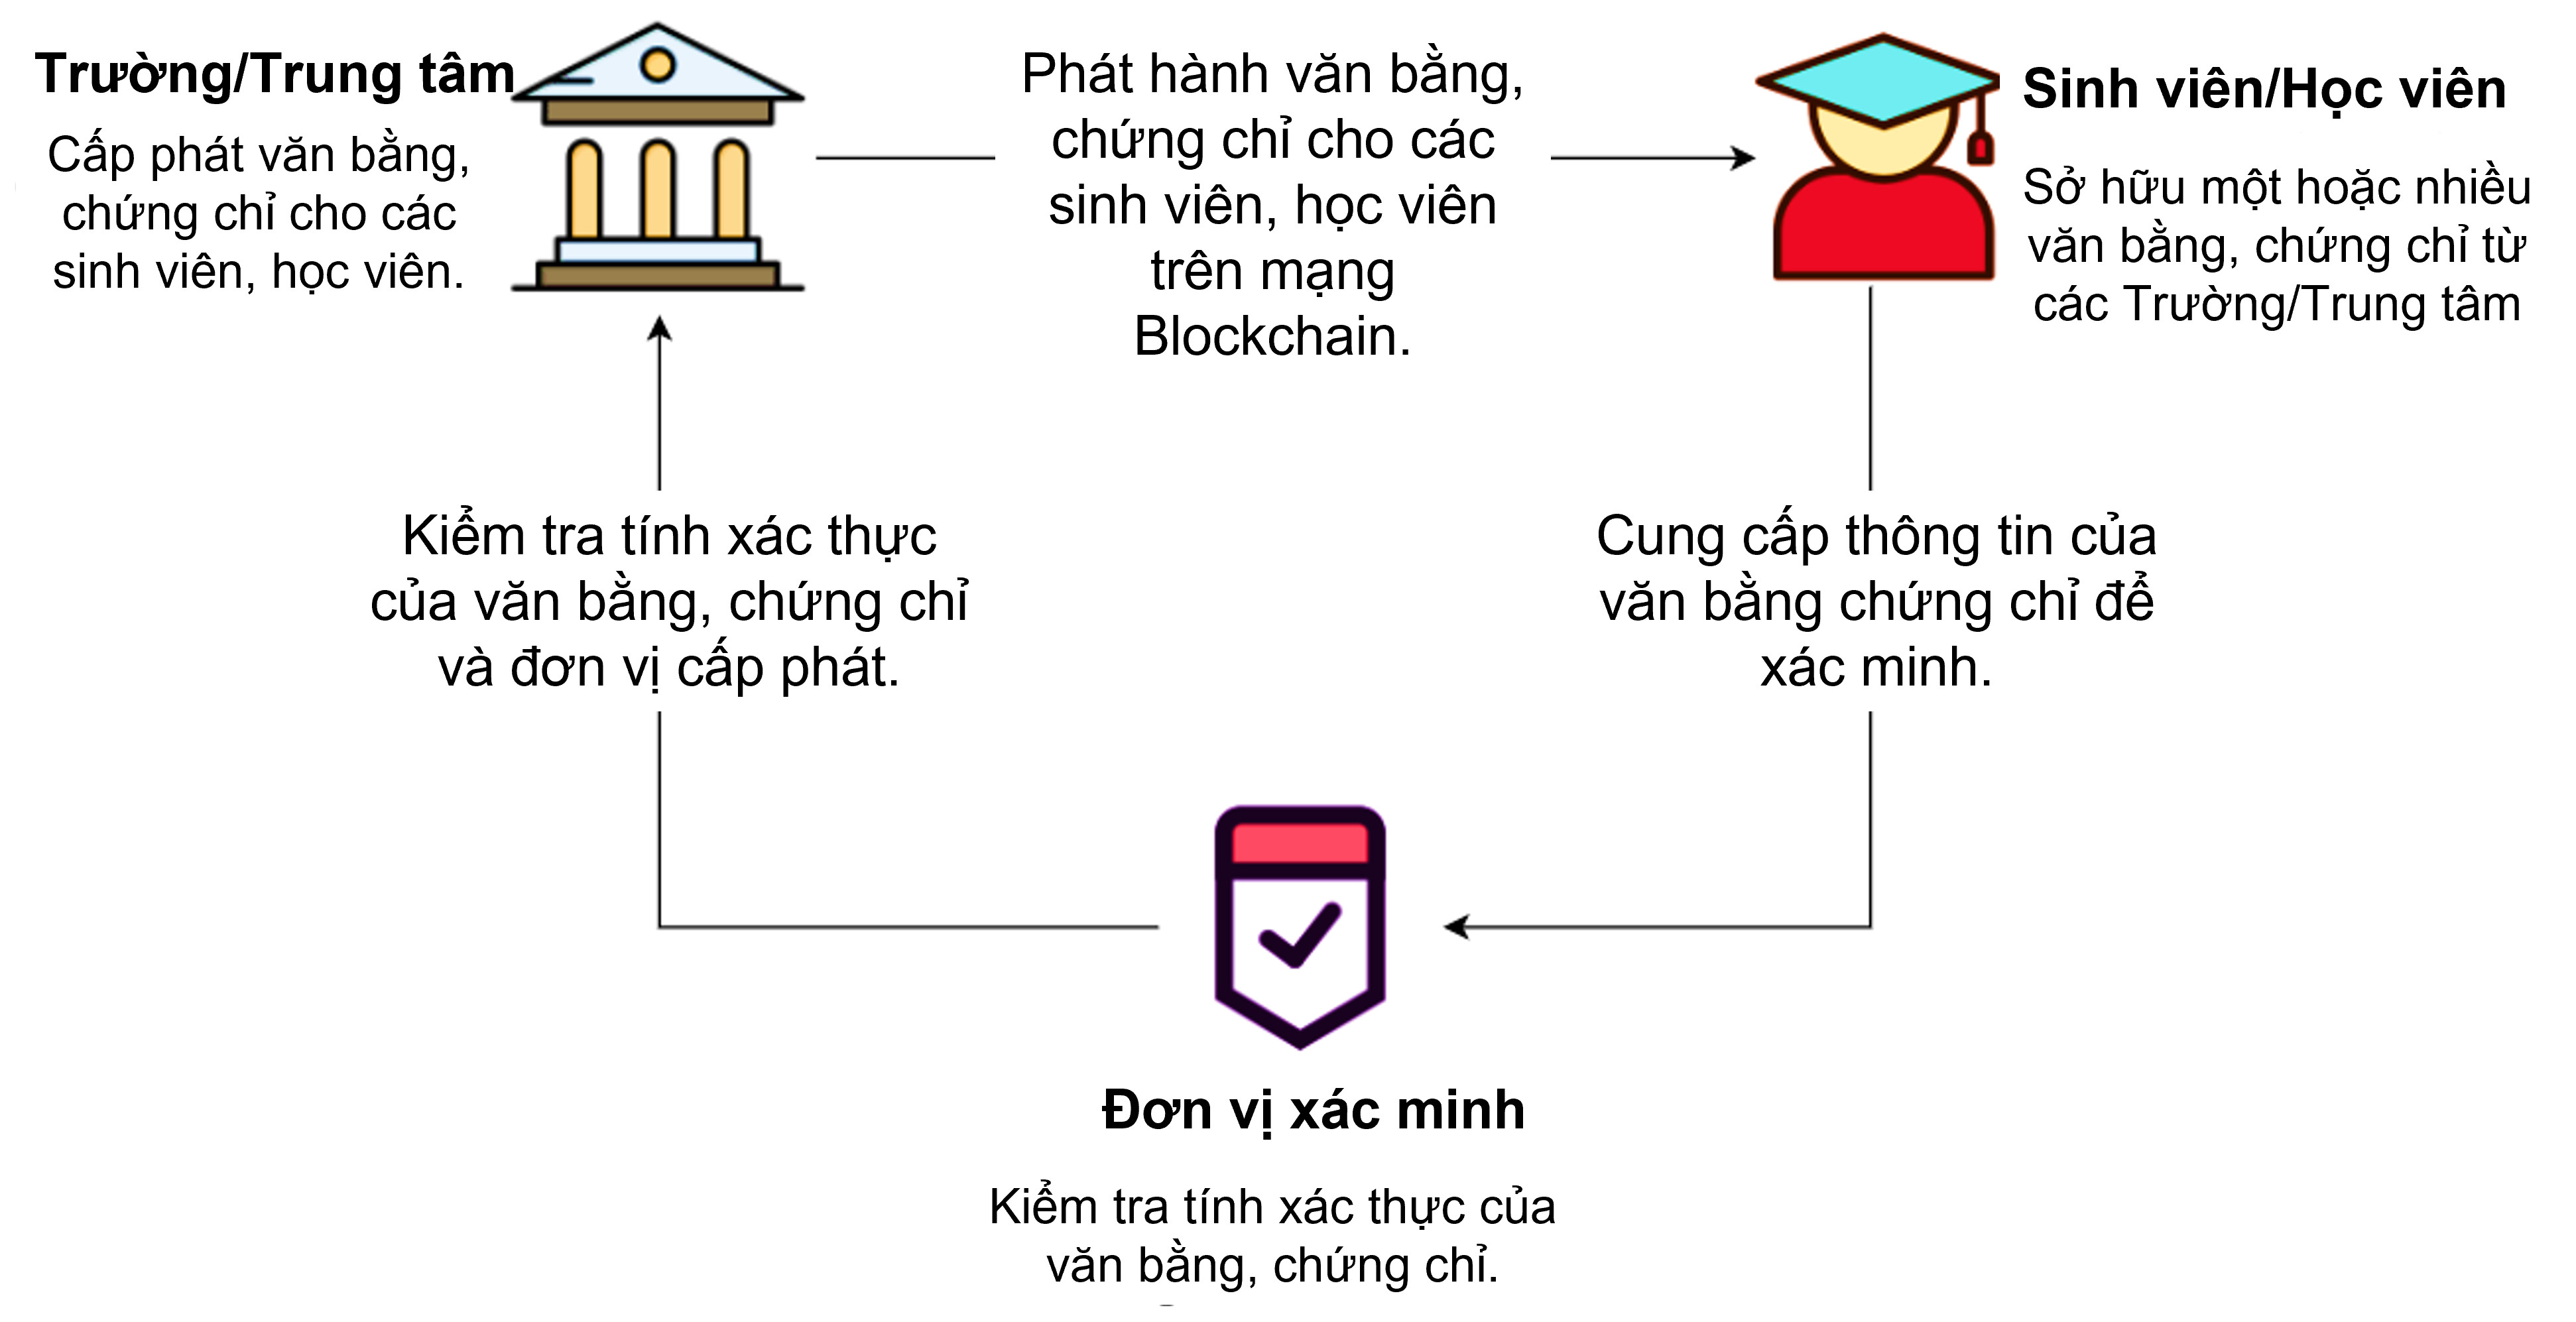
\includegraphics[width=.9\linewidth]{img/vbcc.jpg}
\caption{Sơ đồ bài toán quản lý VBCC ứng dụng blockchain}
\label{fig:vbcc}
\end{figure}

\begin{enumerate}
\item Phát hành VBCC cho sinh viên/học viên:
Thông tin VBCC của sinh viên được lưu trên hệ thống blockchain để đảm bào tính an toàn và tin cậy. Ngoài ra, Trường ký số các thông tin VBCC, nên thông tin VBCC của sinh viên sẽ chống được sự giả mạo trên môi trường điện tử.

\item Cung cấp thông tin xác minh VBCC:
Sinh viên có thể sở hữu một hoặc nhiều VBCC của Trường cấp. Khi cần xác minh VBCC thì chỉ cần gửi thông tin VBCC, có thể lựa chọn thông tin cá nhân như giới tính, dân tộc \ldots khi chia sẻ cho đơn vị xác minh

\item Kiểm tra xác minh VBCC:
Đơn vị xác minh chỉ cần nhận thông tin VBCC được chia sẻ từ sinh viên, sau đó có thể xác thực thông tin VBCC với dữ liệu trong Blockchain.

\end{enumerate}


\section{Tổng quan giải pháp}

Nghiên cứu đề xuất một mô hình thử nghiệm ứng dụng Blockchain để đảm bảo tính an toàn thông tin VBCC và tính bí mật thông tin của người được cấp VBCC.
Hệ thống thực hiện việc ký số khi cấp VBCC, lưu VBCC đã cấp vào blockchain và truy vấn dữ liệu blockchain để xác thực VBCC. 

Hình \ref{fig:vbcc_phanmem} mô tả sơ đồ kiến trúc hệ thống. Trong đó gồm có 3 thành phần chính:

- Phần ứng dụng web: giao tiếp với người dùng, truy vấn, cập nhật dữ liệu vào Blockchain, CSDL

- Phần CSDL: mongoDB để lưu thông tin VBCC và các thông tin không được lưu trong Blockchain.

- Phần Blockchain: để lưu trữ VBCC trên nền tảng Hyperledger Fabric và CA quản lý truy cập người dùng và ứng dụng bằng mật mã khóa công khai.


\begin{figure}[H]
\centering
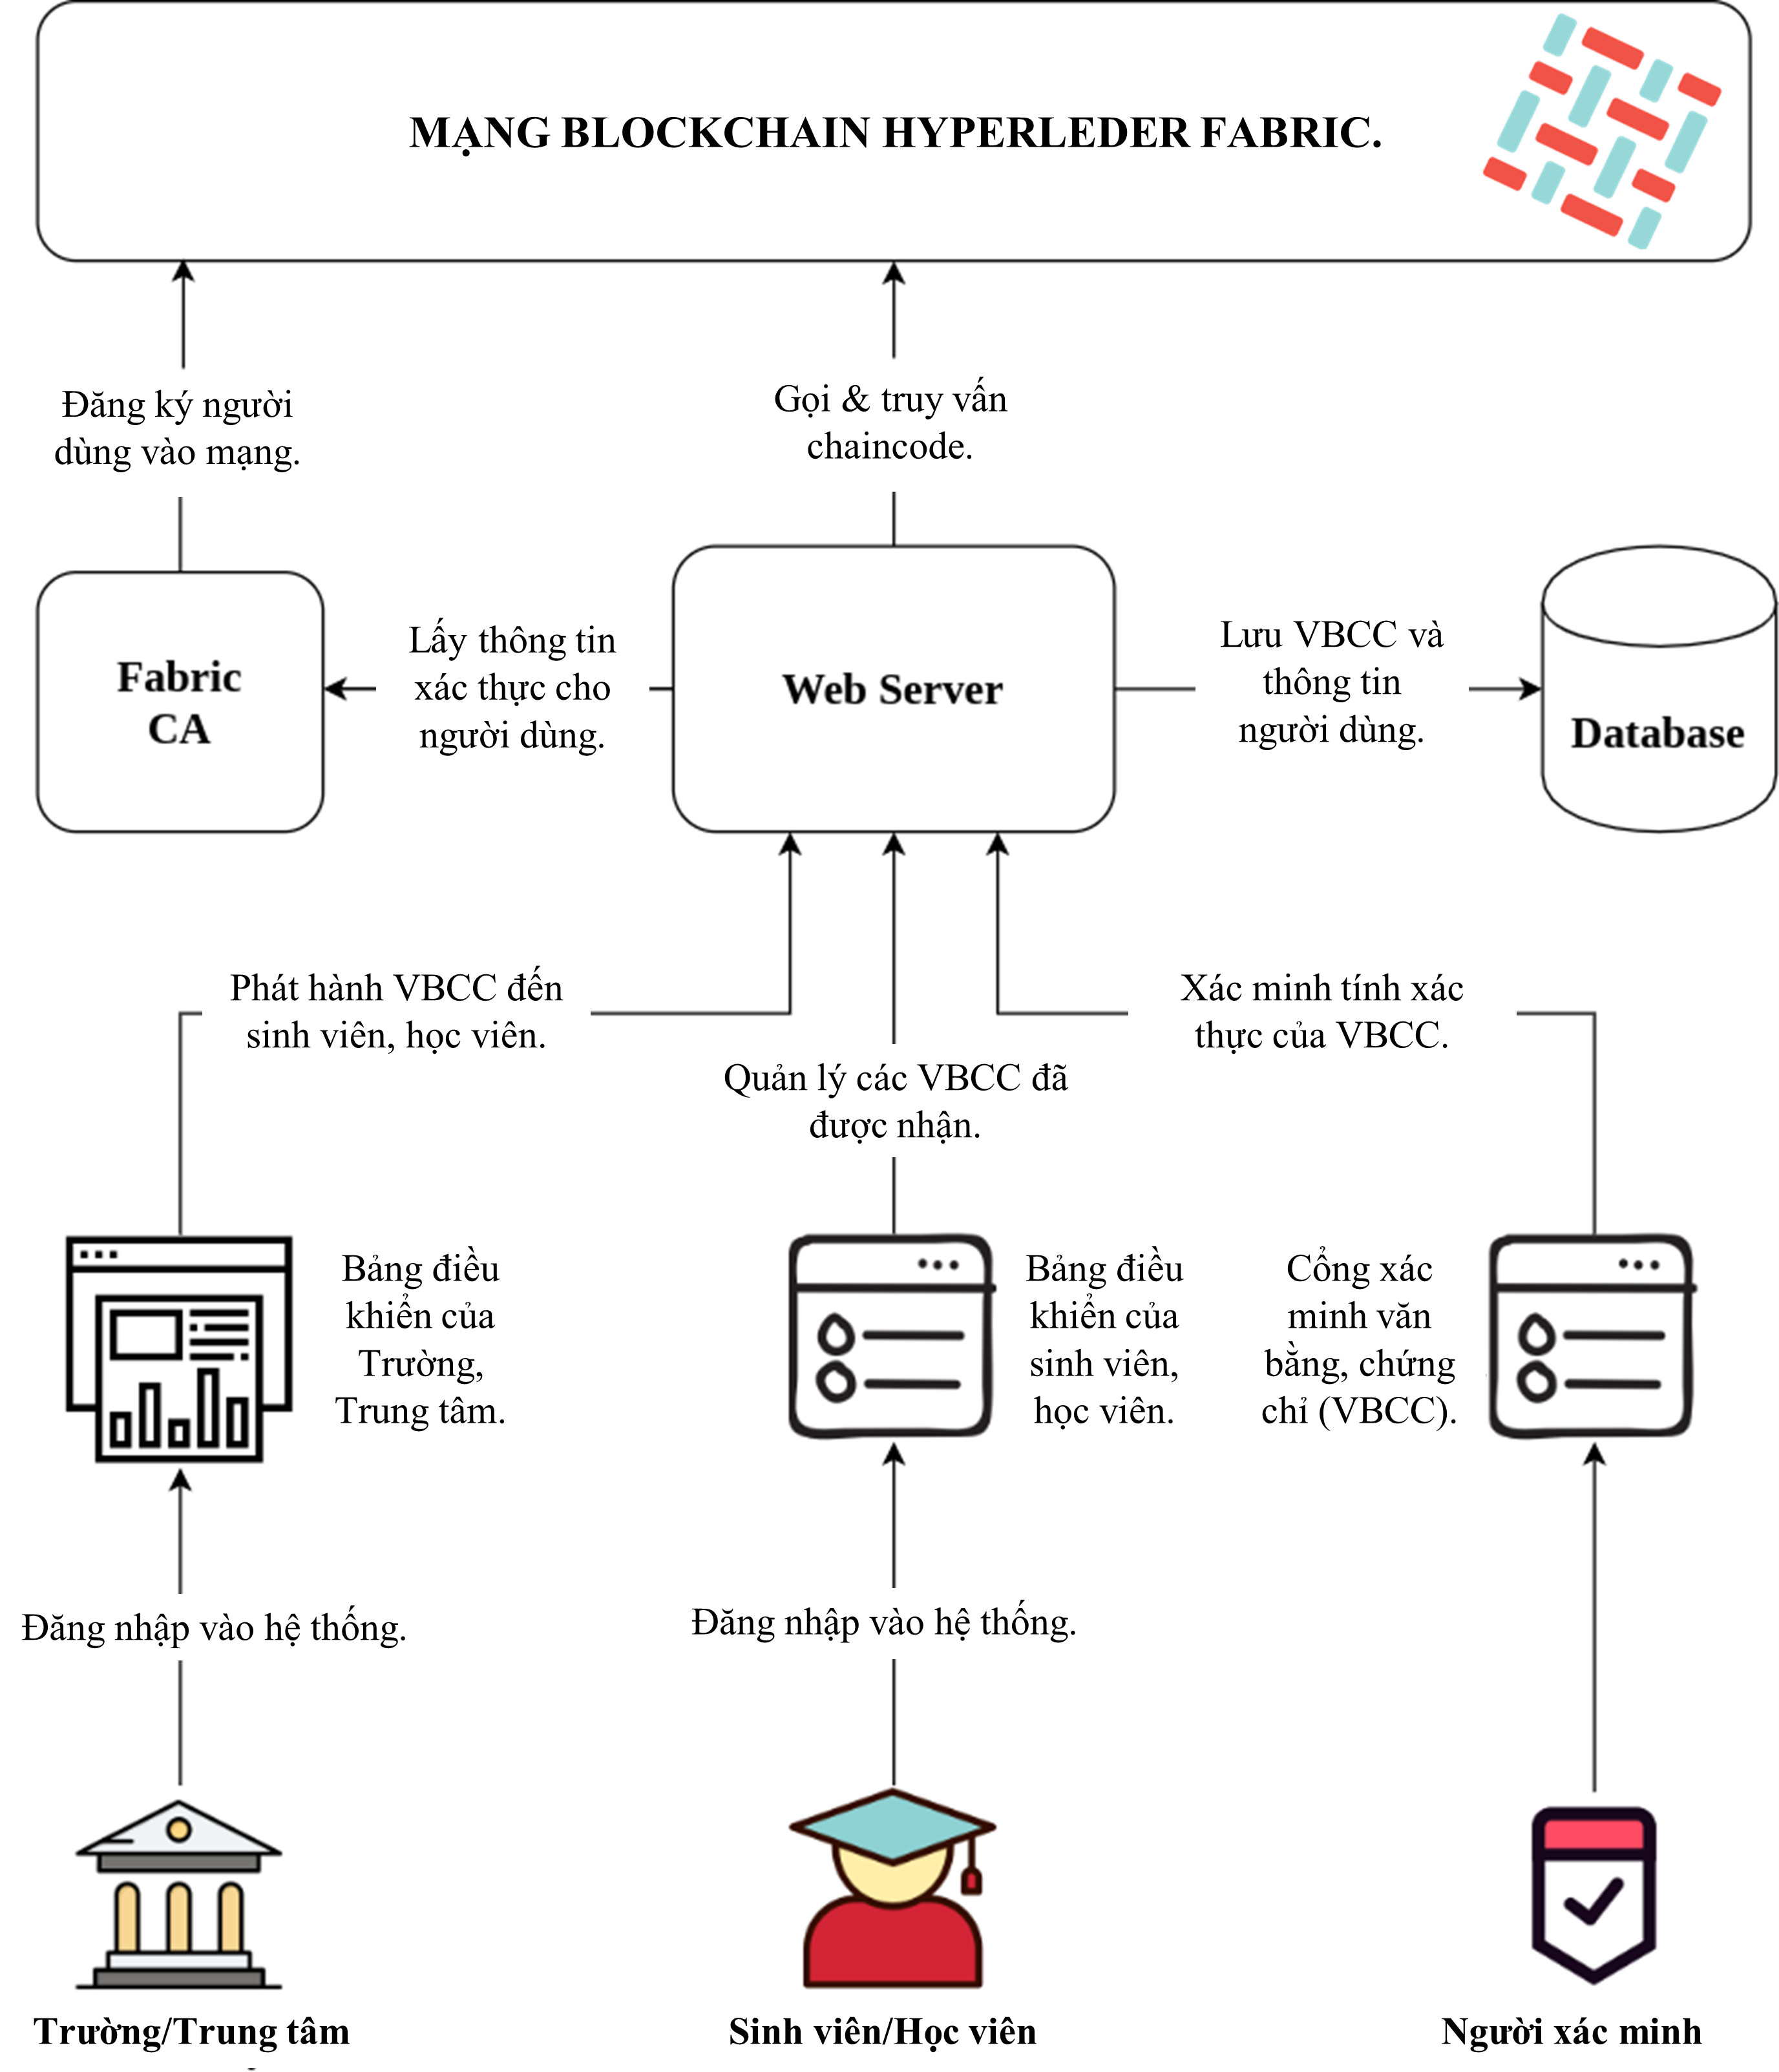
\includegraphics[width=.9\linewidth]{img/vbcc_phanmem.jpg}
\caption{Sơ đồ kiến trúc hệ thống}
\label{fig:vbcc_phanmem}
\end{figure}

Quy trình hoạt động của hệ thống được minh họa như hình \ref{fig:vbcc_diagram}.

\begin{enumerate}
\item Trường phát hành VBCC cho sinh viên/học viên

	\begin{itemize}
		\item 
	Bước 1. Trường đăng ký tài khoản sử dụng hệ thống.
\item 
		Bước 2. Trường điền thông tin đăng ký tài khoản.
	\item
		Bước 3. Trường đăng nhập để sử dụng hệ thống.
	\item 
		Bước 4. Trường chọn chức năng phát VBCC.
	\item
		Bươc 5. Trường nhập thông tin VBCC, số hiệu phôi, số vào sổ gốc, họ tên, ngày sinh, giới tính, nơi sinh, kết quả, ngày cấp, người cấp.
		Trong đó thông tin Email của sinh viên để cần để lấy thông tin khóa công khai dành để ký số với khóa cá nhân của Trường. VBCC được lưu trên Blockchain và chữ ký số của Trường.
	\end{itemize}
\item Sinh viên quản lý VBCC được cấp

	\begin{itemize}
		\item 
	Bước 1. Sinh viên đăng ký tài khoản sử dụng hệ thống.
\item 
		Bước 2. Sinh viên điền thông tin đăng ký tài khoản.
		Trong đó thông tin Email của sinh viên để cần để lấy thông tin khóa công khai để truy cập thông tin VBCC của sinh viên, được lưu trên Blockchain.
	\item
		Bước 3. Sinh viên  đăng nhập để sử dụng hệ thống.
	\item 
		Bước 4. Sinh viên chọn chức năng phát VBCC.
	\item
		Bươc 5. Thông tin VBCC được truy vần từ Blockchain, số hiệu phôi, số vào sổ gốc, họ tên, ngày sinh, giới tính, nơi sinh, kết quả, ngày cấp, người cấp. 
Sinh viên có thể sở hữu một hoặc nhiều VBCC của Trường cấp. 
	\item Bước 6. Sinh viên chia sẻ VBCC với đơn vị xác minh. 
	\item Bước 7. Sinh viên chọn thông tin cá nhân muốn chia sẻ.
	\item Bước 8. Sinh viên gửi thông tin xác minh VBCC cho Đơn vị xác minh VBCC.
	\end{itemize}
\item Đơn vị kiểm tra xác minh VBCC

Đơn vị xác minh chỉ cần nhận thông tin VBCC được chia sẻ từ sinh viên, sau đó có thể xác thực thông tin VBCC với dữ liệu trong Blockchain. Kết quả hợp lệ và không hợp lệ.

\end{enumerate}
\begin{figure}[htbp]
\centering
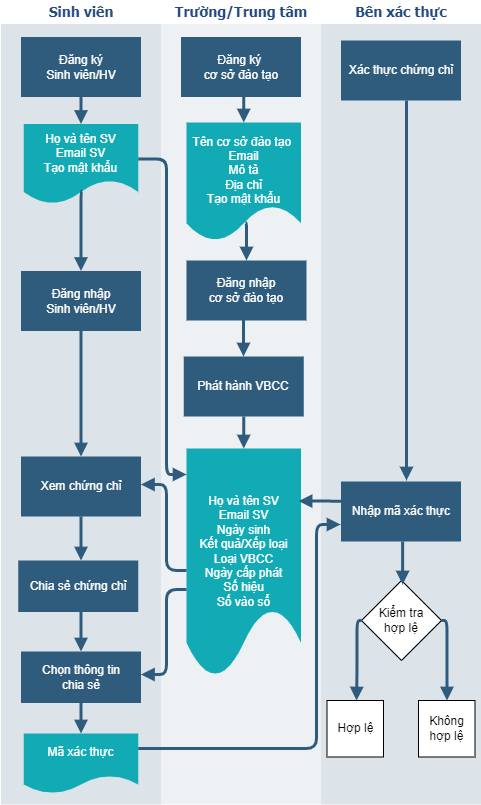
\includegraphics[width=.9\linewidth]{img/vbcc_diagram2.png}
\caption{Quy trình hoạt động của hệ thống}
\label{fig:vbcc_diagram}
\end{figure}

\subsection{Danh sách tác nhân}

\begin{table}[H]
\caption{Danh sách tác nhân}
	\label{table:actor}
	\begin{tabularx} {\textwidth} {|p{1cm}|p{3cm}|X|}
\hline
	ID & Tên actor & Mô tả \\ \hline
	A1 & Sinh viên &  là sinh viên/học viên nhận VBCC \\ \hline
	A2 & Trường học  & Trường/Đơn vị có quyền cấp VBCC \\ \hline
	A3 & Người xác minh  & Người/Đơn vị có nhu cầu xác minh VBCC \\ \hline
\end{tabularx}
\end{table}

\subsection{Danh sách chức năng}

\begin{table}[H]
\caption{Danh sách chức năng}
	\label{table:usecase}
	\begin{tabularx} {\textwidth} {|p{1cm}|p{1cm}|p{3cm}|X|X|}
\hline
		STT &	ID & Tên Use Case & Mô tả & Yêu cầu nghiệp vụ \\ \hline
		1 & U1	& Đăng nhập &Đăng nhập vào hệ thống để xác thực người dùng &Được mở rộng bởi tất cả \\ \hline
		2 & U2 & Đăng ký  & Đăng ký tài khoản vào hệ thống & Được mở rộng bởi tất cả\\ \hline
		3 & U3	&Cấp VBCC & Cấp VBCC có xác nhận chứng thực và ký số VBCC & \\ \hline
		4& U4	& Xem VBCC đã cấp&  Xem các VBCC Trường cấp & \\ \hline
		5 & U5	&Xem VBCC đã nhận & Xem VBCC sinh viên đã nhận& \\ \hline
	6	& U6	&Chia sẻ thông tin VBCC &Chia sẻ thông tin VBCC & \\ \hline
		7& U7	& Xác thực VBCC &Xác minh tính xác thực của VBCC với nền tảng blockchain & \\ \hline
\end{tabularx}
\end{table}

\subsection{Mô tả chức năng hệ thống}
\begin{enumerate}
\item 
Chức năng Đăng ký tài khoản
\begin{itemize}
\item Mô tả: chức năng này cho phép người dùng đăng ký tài khoản để đăng nhập vào hệ thống, để sử dụng các chức năng yêu cầu bắt buộc đăng nhập.
\item Tác nhân: sinh viên, trường cấp VBCC 
\item Yêu cầu: người dùng đã truy cập vào hệ thống 
\end{itemize}

\item 
Chức năng Đăng nhập
\begin{itemize}
\item Mô tả: chức năng để người sử dụng đăng nhập vào hệ thống
\item Tác nhân: sinh viên, trường cấp VBCC
\item Yêu cầu: người dùng đã truy cập vào cập hệ thống
\end{itemize}

\item 
Chức năng Cấp VBCC
\begin{itemize}
\item Mô tả: chức năng cho phép Trường thêm mới một VBCC 
\item Tác nhân: Trường cấp VBCC
\item Yêu cầu: người dùng đã đăng nhập vào hệ thống; người dùng chọn chức năng cấp VBCC
\end{itemize}

\item 
Chức năng Xem VBCC đã cấp
\begin{itemize}
\item Mô tả: chức năng cho phép người dùng xem VBCC đã cấp 
\item Tác nhân: Trường cấp VBCC 
\item Yêu cầu: người dùng đã đăng nhập vào hệ thống; người dùng chọn chức năng xem VBCC
\end{itemize}

\item 
Chức năng Xem VBCC đã nhận
\begin{itemize}
\item Mô tả: chức năng cho phép người dùng xem VBCC 
\item Tác nhân: sinh viên
\item Yêu cầu: người dùng đã đăng nhập vào hệ thống; người dùng chọn chức năng xem VBCC
\end{itemize}

\item 
Chức năng Chia sẻ thông tin VBCC
\begin{itemize}
\item Mô tả: chức năng cho phép người dùng chia sẽ thông tin VBCC 
\item Tác nhân: sinh viên 
\item Yêu cầu: người dùng đã đăng nhập vào hệ thống; người dùng chọn chức năng chia sẽ VBCC
\end{itemize}

\item 
Chức năng Xác thực VBCC
\begin{itemize}
\item Mô tả: chức năng cho phép người dùng xác thực VBCC
\item Tác nhân: người xác minh, sinh viên, trường 
\item Yêu cầu: người dùng truy cập vào hệ thống; người dùng chọn chức năng xác thực VBCC
\end{itemize}

\end{enumerate}

\subsection{Thiết kế CSDL}

Danh sách cấu trúc dữ liệu trong hệ thống


\begin{table}[H]
\caption{Danh sách cấu trúc dữ liệu trong hệ thống}
	\label{table:dataschema}
	\begin{tabularx} {\textwidth} {|p{1cm}|p{3cm}|X|}
\hline
		STT &	Tên cấu trúc & Diễn giải \\ \hline
		1 & certificate	& Cấu trúc thông tin VBCC\\ \hline
		2 & student & Cấu trúc thông tin sinh viên \\ \hline
		3 & university	&Cấu trúc thông tin trường/trung tâm \\ \hline
	\end{tabularx}
\end{table}

Thuộc tính của các cấu trúc dữ liệu

\begin{table}[H]
\caption{Bảng mô tả các thuộc tính của cấu trúc certificate}
	\label{table:certificate}
	\begin{tabularx} {\textwidth} {|p{1cm}|p{3cm}|p{3cm}|X|p{2cm}|}
\hline
		STT &	Tên trường & Kiểu dữ liệu & Diễn giải & Ràng buộc \\ \hline
		1 & studentName	& String & Họ tên  & not null \\ \hline
		2 & studentEmail & String  & Email   & not null \\ \hline
		3 & studentID	&  String & Mã số  & not null\\ \hline
		4 & birthday	& String & Ngày sinh & not null\\ \hline
		5 & place	& String & Nơi sinh & not null\\ \hline
		6 & gender & String & Giới tính & not null\\ \hline
		7& ethnic	& String & Dân tộc & not null\\ \hline
		8& universityName	& String & Tên trường cấp VBCC & not null \\ \hline
		9& universityEmail	& String & Email trường cấp VBCC&not null\\ \hline
		10& major 	& String & Khóa  học  & not null\\ \hline
		11& number	& String & Số hiệu VBCC & not null\\ \hline
		12& regNo	& String & Số vào sổ gốc & not null \\ \hline
		13& departmentName	& String & Tên khoa &\\ \hline
		14& cgpa	& String & Kết quả & not null \\  \hline
		15& dateOfIssuing	& String & Ngày cấp &not null\\ \hline
		
\end{tabularx}
\end{table}


\begin{table}[H]
\caption{Bảng mô tả các thuộc tính của cấu trúc student}
	\label{table:student}
	\begin{tabularx} {\textwidth} {|p{1cm}|p{3cm}|p{3cm}|X|p{2cm}|}
\hline
		STT &	Tên trường & Kiểu dữ liệu & Diễn giải & Ràng buộc \\ \hline
		1 & email	& String & Email  & not null \\ \hline
		2 & name & String  & Họ tên   & not null \\ \hline
		3 & password	&  String & Mật khẩu  & not null\\ \hline
		4 & publicKey	& String & Khóa công khai  & not null\\ \hline
\end{tabularx}
\end{table}


\begin{table}[H]
\caption{Bảng mô tả các thuộc tính của cấu trúc university}
	\label{table:university}
	\begin{tabularx} {\textwidth} {|p{1cm}|p{3cm}|p{3cm}|X|p{2cm}|}
\hline
		STT &	Tên trường & Kiểu dữ liệu & Diễn giải & Ràng buộc \\ \hline
		1 & email	& String & Email  & not null \\ \hline
		2 & name & String  & Tên trường   & not null \\ \hline
		3 & location	&  String & Địa chỉ  &not null \\ \hline
		4 & password	& String & Mật khẩu  &not null \\ \hline
		5 & publicKey	& String & Khóa công khai   &not null \\ \hline
\end{tabularx}
\end{table}

\subsection{Thiết kế blockchain}
\begin{enumerate}
\item 
Danh sách các đối tượng trong hệ thống


\begin{table}[H]
\caption{Danh sách các đối tượng trong hệ thống}
	\label{table:asset}
	\begin{tabularx} {\textwidth} {|p{1cm}|p{3cm}|X|}
\hline
		STT &	Tên cấu trúc &  Diễn giải \\ \hline
		1 & certificate	& Chứng chỉ  \\ \hline
		2 & schema  &  Loại VBCC  \\ \hline
		3 & university	&  Trường cấp VBCC  \\ \hline
\end{tabularx}
\end{table}

\begin{table}[H]
\caption{Bảng mô tả các thuộc tính của đối tượng certificate}
	\label{table:assetcertificate}
	\begin{tabularx} {\textwidth} {|p{0.8cm}|p{3.5cm}|p{2.5cm}|X|p{2cm}|}
\hline
		STT &	Tên trường & Kiểu dữ liệu & Diễn giải & Ràng buộc \\ \hline
		1 & certHash	& String & Lưu giá trị băm của VBCC  & not null \\ \hline
		2 & universitySignature & String  & Chữ ký số lên certHash dùng khóa cá nhân của Trường cấp VBCC  & not null \\ \hline
		3 & studentSignature	&  String & Chữ ký số lên certHash dùng khóa cá nhân của sinh viên nhận VBCC  & not null\\ \hline
		4 & dateOfIssuing	& String & Ngày cấp  &not null \\ \hline
		5 & certNumber	& String & Số hiệu VBCC  & not null\\ \hline
		6 & certRegNo	& String & Số vào sổ gốc  & not null\\ \hline
		7 & certNumber	& String & Số hiệu VBCC  & not null\\ \hline
		8 & certUUID	& String & Mã số VBCC  & not null\\ \hline
		9 & universityPK	& String & Khóa công khai của Trường cấp VBCC  &not null \\ \hline
		10 & studentPK	& String & Khóa công khai của sinh viên nhận VBCC  &not null \\ \hline
\end{tabularx}
\end{table}


\begin{table}[H]
\caption{Bảng mô tả các thuộc tính của đối tượng schema}
	\label{table:assetschema}
	\begin{tabularx} {\textwidth} {|p{1cm}|p{3cm}|p{3cm}|X|p{2cm}|}
\hline
		STT &	Tên trường & Kiểu dữ liệu & Diễn giải & Ràng buộc \\ \hline
		1 & certificateType	& String & Loại VBCC  & not null \\ \hline
		2 & id  & String  & Mã loại  & not null \\ \hline
		3 & ordering	&  String &   & \\ \hline
	\end{tabularx}
\end{table}


\begin{table}[H]
\caption{Bảng mô tả các thuộc tính của đối tượng university}
	\label{table:assetuniversity}
	\begin{tabularx} {\textwidth} {|p{1cm}|p{3cm}|p{3cm}|X|p{2cm}|}
\hline
		STT &	Tên trường & Kiểu dữ liệu & Diễn giải & Ràng buộc \\ \hline
		1 & name	& String & Tên Trường cấp VBCC  & not null \\ \hline
		2 & publicKey & String  & Khóa công khai của Trường cấp VBCC  & not null \\ \hline
		3 & location	&  String & Địa điểm  &not null \\ \hline
		4 & description	& String & Thông tin mô tả  &not null \\ \hline
\end{tabularx}
\end{table}

\end{enumerate}
